
One of the most important mechanisms in XtreemFS is the possibility to have
several replicas of a file distributed over the Grid. This feature affords
data-intensive applications achieving better performance as long as: there is no
single access point for the data and mechanisms for parallel access can be
exploited. Besides, replication also provides reliability and availability to
the filesystem, which is of vital importance for a distributed environment.

However, the usage of Grid resources such as network (where data is transfered
across) or storage (where data is stored) are finite, shared, and non-free.
Furthermore, the synchronization of the replicas of any given file involves
additional overheads, so that mechanisms that keep the tradeoff between the
benefits and the extra costs are needed.

For aiming at all of these purposes, we are working on the implementation of the
Replica Management Service. This service concerns about: selecting the best
replicas for the applications, creating and deleting replicas automatically
taking account of how and from where they are accessed and evaluating the
maximum number of replicas of any given file.


\subsection{Choosing the best replica}
\label{RMS_Choosing_Replicas}

When a given client (or an OSD) has to access a file, the question is: which
replica should it access? It should be able to detect which replica will provide
better performance. The idea to solve this problem is to build a virtual 2D
space and locate all replicas, OSDs, and clients in it. The distance
between two different objects (i.e replica, OSD, or client) is an indicator of
the distance (performance wise) of these two objects. Once a client wants to
access a file, it just needs to compute the euclidian distance between itself
and all replicas and choose the closer one.

\subsubsection{Vivaldi Algorithm}

Vivaldi is a light-weight algorithm developed by MIT \cite{dabek2004vdn} 
that allows assigning a position in a coordinate space to every node in a network,
so the distance between the coordinates of two nodes predicts the real communication
latency between them.

In order to generate a valid coordinate system, it is necessary to determine
which space will be used and which formula will be used to calculate the
distance between two given points. In our case, it is been proved that
implementing a 2-D space, where the Euclidean distance between two coordinates
accurately predicts the latency between their corresponding nodes, generates
valid results with a really small error probability.

For the algorithm to work correctly, it is also necessary that the nodes of the
system keep contacting themselves randomly and indefinitely to re-adjust their
position, so any possible change in the network may be reflected. In each
re-adjustment, a node contacts a different neighbor, gets its coordinates and
modifies its own coordinates, so eventually the Euclidean distance is as similar
as possible to the measured round trip time.

On the other hand, once a group of nodes have established a valid coordinate
system, it is necessary to use some mechanism that helps to reduce the impact of
introducing new nodes, so we avoid them to alter the already stabilized system.
That is why Vivaldi keeps in every node, besides the coordinates, a local error
that informs about how sure a node is about its position. This way, a node with
a steadier position will have a smaller local error and will influence more the
rest of nodes when they contact it to readjust their position (figure
\ref{rms1}).

\begin{figure}[t]
\begin{center}
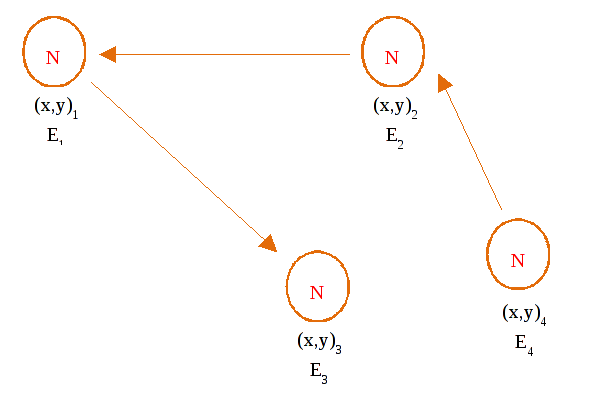
\includegraphics[width=0.60\textwidth]{images/rms1.png}
\caption{Nodes keep recalculating their position}
\label{rms1}
\end{center}
\end{figure}

Once the system is adjusted, any node of the network can determine which nodes
are the closest ones with a really simple calculation, in a very short period of
time and without generating extra traffic.

Some already developed implementations of Vivaldi can be found in p2psim and in
Chord. You might also be interested in Ledlie et al.'s work \cite{ledlie2007ncw}.

\subsubsection{Vivaldi in XtreemFS}

As we have different kinds of nodes in our architecture, not all of them work in
the same way to integrate Vivaldi. While the clients usually execute during
shorter periods of time, the servers are up and running , so the
idea is to let the OSDs (at this moment they are the only
servers that implement Vivaldi) establish a permanent coordinate system where a
client can move through, to find its position.

\subsubsection{Vivaldi in the OSDs}

An OSD has an independent stage responsible of managing Vivaldi on its side and
of providing to the rest of components a couple of valid coordinates that define
the position of the node in the current coordinate system.

The stage keeps running indefinitely and periodically contacts a different OSD
to ask it for its coordinates and its local error. With that data and the
coordinates of the own OSD is possible to compute the Euclidean distance and to
compare it with the real RTT measured against the contacted node.

The frequency an OSD readjusts its position is defined by the parameters
MIN\_\-TIMEOUT\_\-RECALCULATE and MAX\-\_TIMEOUT\_\-RECALCULATE. Just after performing a
readjustment, the stage typically calculates a random number included in the
interval of time defined by those two parameters and sleeps during that number
of seconds until the next iteration. This way we try to avoid generating traffic
peaks where all the nodes send a request at the same time and to distribute the
net use in time.

Larger periods will reduce the overhead in the network but will make the nodes
to adjust more slowly to the possible changes in the environment, while smaller
ones will require more traffic but will produce a more reactive system.

In each iteration, the introduced stage chooses a node to contact to from a list
of available OSDs, which is filled with the information contained in the
Directory Service. This list must be updated somehow so the stage can always
notice a node going offline.

\subsubsection{Vivaldi in clients}

In our system, the clients usually execute during a much shorter period of time,
so they have to be able to determine their position faster. This can be done
because they do not influence the rest of the nodes and they just take some
needed info from the already placed OSDs to locate themselves.

In Vivaldi, each node is responsible for its own coordinates and typically has to
recalculate them at least a small number of times before they represent the real
position in the coordinate system. Even if the set of OSDs is``adjusted'', a
client will need to recalculate its position (against one single node each time)
several times before having an accurate approximation of its real location.
Vivaldi requires that the nodes of the net generate traffic and communicate
among themselves.

As in the case of the OSDs, a client also has the parameters
MIN\_\-TIMEOUT\_\-RECALCULATE and MAX\_\-TIMEOUT\_\-RECALCULATE that allow defining the
recalculation period. Although the analogue parameters in the OSDs have the same
names, they are different parameters and therefore they all must be defined in
different files.

Finally, it is important to emphasize that after the first boot of the client,
it keeps its coordinates and preserves them among executions, so it remains well
located though it mounts and unmounts a lot of different volumes or opens and
closes a lot of files. The coordinates are not reinitialized until the client
node is rebooted.

\subsubsection{Replica Selection with Vivaldi}

Until this point we have introduced a mechanism able of establishing a
coordinate system where all the nodes of a network have a pair of coordinates
that allows them predicting the round trip time to the rest of neighbors. Now it
is time to analyze how to take advantage of that information and to describe the
current applications of Vivaldi in XtreemFS.

Sometimes during the execution of certain operations, the client has to choose
which replica access, among several replicas stored in different nodes of the
system. The ideal solution proposes to select always the replica that is stored
in the closest node, so the accesses can be made within the minimum time. But
the problem is that most of the times measuring the RTT against every OSD, for
each selection, is not computationally feasible.

Using the coordinates provided by Vivaldi, a client can calculate which replica
is the closest one with a practically insignificant delay. At this point the
only remaining problem seems to be how to gather all the coordinates so they can
be available in the exact moment of the replica selection.

As mentioned earlier, in Vivaldi the coordinates are managed
independently by the node they belong to and remain distributed among the
different nodes of the network. In order to let the client take advantage of
them, it is necessary to collect them in the MRC, so they can be included in
every list of x-locations.

\begin{figure}[t]
\begin{center}
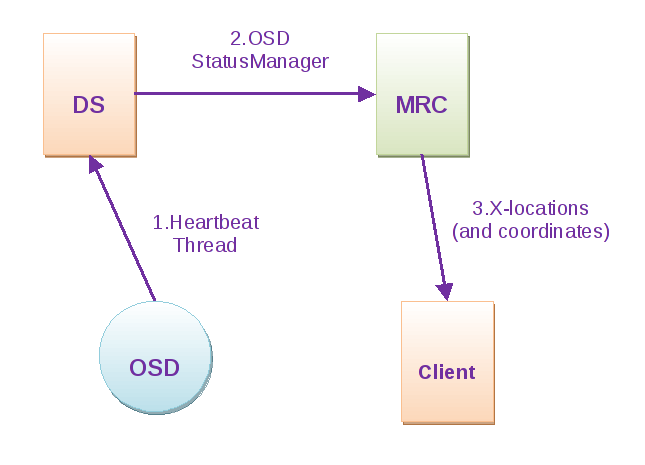
\includegraphics[width=0.60\textwidth]{images/rms2.png}
\caption{Collecting the coordinates}
\label{rms2}
\end{center}
\end{figure}

In figure \ref{rms2} we show the following process:

\begin{enumerate}
\item HeartbeatThread is a component of the OSDs that periodically registers the
OSD in the Directory Service. The information that is uploaded each time is
determined by the function getServiceData, which is defined in the main
constructor of the class OSDRequestDispatcher.
\item OSDStatusManager is a component of the MRC that regularly queries the
Directory Service for available OSDs.
\item During an open operation, the MRC sends to a client a list of x-locations,
so it can locate the different replicas associated to a certain file. The
x-locations include the corresponding coordinates, so the client can use them to
predict the closest replica.
\end{enumerate}


\subsection{Replica creation}
\label{RMS_Replica_Creation}

Another important issue regarding replicas is to decide when and where to create
a replica. For this functionality we have three different mechanisms. The first
one is an explicit request from the user. In this scenario, the RMS will not
take any action. The second one is a reactive replica creation. The system will
detect that a replica is needed at a given location and will start a replica
creation. Finally, in the third case, the system will predict the usage of a
file in a location where no replicas are nearby and thus will try to create the
replica before it is used. We call to this third mechanism proactive replica
creation.

In both cases reactive and proactive, we plan to provide a mechanism able to
study the access pattern of files and use it to decide if only a part of the
file needs to be replicated (partial replication). This partial replicas will
speedup the process of replication because only part of the data will need to be
copied to the new location. Nevertheless if we miss-predict the parts of the
replica that will be used, we will always be able to populate the missing parts
on-demand (done directly by the OSDs).

%TODO: We could increase the level of detail in following subsubsections
\subsubsection{Reactive replica creation with Vivaldi} 

In this scenario it is detected when replicas are currently needed in other
parts of the Grid. Then, using the distance mechanisms we just described in
Section \ref{RMS_Choosing_Replicas}, we will detect if clients request a replica
from large distances. So in this case Vivaldi could be used to decide a better
location for a replica and create it.

\subsubsection{Proactive replica creation with Oraculo}

We have implemented a service called Oraculo that carries out data mining on
multi-order context models to analyze the file-access patterns and to compute
future accesses. For the implementation of such multi-order context models,
Oraculo keeps a trie (or prefix tree) as Kroeger et al. did \cite{kroeger1996pfs,
kroeger2001dai} for centralized environments, where they proved that such structures
where effective. 

Thus, each file access is modeled as a symbol (i.e. the file path) and it is
recorded as a node of the prefix tree with an associated value that represents
how many times the chain pattern from root to that node has ocurred.

Then, in order to interact with Oraculo, it provides a basic interface for:
\begin{enumerate}
 \item Adding an event to the trie, given a sequence of the last events seen.
 \item Getting a prediction from the trie, given a sequence of the last events
seen.
\end{enumerate}

So that when a file access is produced, it can be noticed to Oraculo which
computes which parts of the trie must be modified, adding the new event to the
corresponding branches or simply increasing the counter of the pattern if it is
already present.

Notice that in order to keep the trie scalable Oraculo can prune it in two ways.
First, keeping a predefined maximum number of nodes per branch. Thus, whenever a
new event goes to a full branch all its nodes divide their corresponding value
by two and nodes with a value lower than 1 are deleted from the trie. In the
case that no node has been cleaned, the new event is not added. But, obviously
the nodes in the branch keep the new value (after the division by two) so in the
near future it will be eventually possible to add new events in that branch.

On the other hand, Oraculo also has a maximum of root-branches (also called
partitions) to keep the horizontal scalability of the trie. Here we apply a
LRU-based algorithm among the partitions taking account of their usage as well.

Finally, Oraculo can predict future file accesses by applying basic data-mining
on the trie. It only needs to know some previous accesses to look for patterns
based on them. Then, an OSD could eventually use this information to replicate
data in advance.

Furthermore, we will propose a decoupled and off-line aggregation of the tries.
Once in a while (still to be determined), OSDs could contact other OSDs (only a
small subset) to exchange their trie information and build an aggregated one
that has the information of all. This mechanism will allow all OSDs to have a
more or less global view because what is learned by one OSD will be propagated
though several aggregations. We have done some preliminary tests using this
mechanism and seems to work very well with environments of many thousands of
nodes.

Regarding the information of the access pattern of files, in most cases the
information kept by a single OSD will be enough. Nevertheless, whenever we need
the full information of the pattern, we can contact all OSDs that have a replica
and aggregate the learned behavior. As we do not expect to keep many replicas of
a file, this procedure seems reasonable and scalable.

\subsubsection{Integration of Oraculo with OSDs}

Unfortunately, the integration of Oraculo with OSDs could not be done yet
because we are still evaluating it by using GridSim (a well-known Grid
simulator). Once we get significant results with the simulations we will
evaluate them and port Oraculo to the OSDs.


%%WARNING: This subsection is copy pasted from D3.4.4
%\subsection{Automatic setting of the number of replicas}
%\label{RMS_replica_limitation}

%The problem of having many replicas is that updates imply that a coordination
%mechanisms has to be started. This coordination will reduce performance and the
%magnitude clearly depends on the number of replicas available. For this reason
%we have decided to set a limit in the number of replicas a file will have.

%On the other hand, it is clear that the overhead this coordination will imply
%also depend on the frequency at which files are modified. For instance, if a
%file is only modified once a month (and only small modification are done) we
%could keep many more replicas than for a file that is constantly modified.

%The objective of this mechanism is to detect the access pattern of files and
%find the ratio between reads and writes. With this information the RMS will
%decide the maximum number of replicas that obtains a good tradeoff between the
%benefit of multiple replicas in read operations and the penalty of coordination
%in write operations.


%%WARNING: This subsection is copy pasted from D3.4.4
\subsection{Replica deletion}
\label{RMS_Replica_Deletion}

On the one hand, if we want to be able to replicate files whenever needed but
still maintain the maximum number for replicas per file, it would be interesting
to keep the number of replicas a bit smaller than the maximum. This difference
between the maximum and the real number of replicas would allow the system to
create replicas whenever needed. On the other hand, if replicas are not used, it
would also be nice to have them removed automatically to reduce disk usage in a
given node and/or center.

To tackle these two issues we will implement a mechanism that automatically
deletes the less important replicas. To know what replicas are less important we
will use similar mechanisms than the ones used to create replicas. We will
predict future usage using the same kind of tries. In addition we will perform
some kind of preventive removal of replicas, which means that whenever a node
decides to remove a replica it will inform other OSDs that have it to react
accordingly.


%%WARNING: This subsection is copy pasted from D3.4.4
\subsection{Interaction with the Application Execution Management}
\label{RMS_AEM_interaction}

The last mechanisms that we will implement to manage replicas consists of an
interaction with the application execution management system (AEM). This
interaction will be done in two steps.

Firstly, AEM analyzes the JSDL of the application and asks to XtreemFS
for the locations (coordinates X,Y) of its files' references. Thus AEM computes
an optimal coordinate around where the job should be executed. This coordinate
is used for AEM to send a request to Resource Selection Service (RSS) for a set
of nodes close to it. Of course, RSS also considers other requirements, such as
CPU or memory, to decide the resulting set of nodes.

In the second step, the AEM will inform XtreemFS on the final destination of a
given job and the files it will use. With this information, the RMS will decide
if new replicas need to be created to improve the I/O performance of this job.
In addition, and in some cases, it might be that the RMS decides to advance this
step from the information obtained in step 1. For instance, this may happen when
the list is made of nodes that are close among themselves and one or two
replicas could do the job.

Although this mechanism is very good in the sense that no prediction needs to be
done, it has a couple of limitations. The first one is that the AEM might not
know the files used by a job (it is not a requirement in the job description).
The second one is that there might not be enough time from the moment XtreemFS
receives the execution location of a job (and the files it uses) and the moment
the job starts running. To solve these two cases we have proposed the previous
prediction mechanisms (\ref{RMS_Replica_Creation}).
